
\documentclass[11.5pt]{article}
\usepackage[margin=1in]{geometry}
\usepackage{hyperref}
\usepackage{amsmath}
\usepackage{verbatim}
\usepackage{graphicx}
\usepackage{bbm}

\title{Make Music Genre Identification Great Again}
\author{Hyeonjung Ko, Yash Shetty}

\date{December 14th, 2019}

\begin{document}

\maketitle

\abstract
Classifying raw music files into distinct genres is a challenging task with numerous practical applications. With the goal of finding the best performing music genre identification model, this project applied 4 well-known classification models to the task, including Support Vector Machine(SVM), Random Forest, Feedforward Neural Network(FNN) and Convolutional Neural Network(CNN). The process was split into three parts: the raw implementation of the models using the Spotify song features, the implementation of CNN using audio spectrogram and the application of the extracted features from CNN to train other classification model types. The classifiers showed poor performance during the first phase and increased in performance under the extracted features from the CNN.\\
\vspace{2mm}
\section{Introduction}
%Describe the problem you are addressing. Be precise in defining the problem. Describe why the problem is important and in what applications it will be useful.

Music has been always been a crucial part of human function. The creation and enjoyment of music has addressed our desire for creativity and emotional satisfaction. With such a wide appreciation for music, the global music industry was valued at estimated \$19.1 billion USD in 2018. Music streaming giants such as Spotify and Youtube strive to hold on to existing users and gain new ones. In this context, companies making a profit based on music streaming and users who consume their products have the need to search for and provide new enjoyable content. Music genre classification provides a part solution for such problems. The genre classifiers allow pattern identification, artist recommendation, and individual curation of content.

The extent of music genre classification models lies far beyond the music industry. The potential to accurately classify audio files can be used for a wide range of other industries including speech processing and environmental sound classification. Specifically in environmental sound classification, the classifiers could be modified to be used as applications for content-based multimedia indexing and retrieval, deaf individuals assistance in daily activities, home security in smart home devices, and predictive maintenance of industrial equipment. 

\section{Technical Approach}
%Describe the techniques you have used in order to address the problem. Describe in detail the classification/regression/other techniques you have used in order to tackle the problem.
In this project, the task was to compare different supervised learning classification models and learn the highest performing classification model for music genre classification.  Four different classification models–SVM, Random Forest, FNN and CNN–were developed in the task of music genre classification given song features or an audio file. The project was split into three parts: the implementation of the models using the Spotify song features, the implementation of CNN using audio spectrogram and the application of the extracted features from CNN to train other classification model types.
 
The approach of SVM was to maximize the margin between the decision boundary and data points. With multiple classes, the SVM model determined multiple decision boundaries using the one vs one approach. Random Forest classifier used the bagging method which merges multiple simple decision trees trained against a given dataset to output a prediction. Its output was the mode of the classes. It searched for the best feature among a subset of the given features. FNN was a sequence of dense, fully connected layers, meaning each node in layer $l$ is connected to every node at layer $l + 1$. The input features were fed forward through the network. At each node, an activation function was applied to the weighted sum of inputs such that the output of the network was a complex, nonlinear function. 

CNN model was used to tackle music genre classification with an alternative approach. Instead of classifying the raw audio data of the given file, it was first transformed into its Mel-frequency cepstral coefficients (MFCC) values to approach it as an image classification problem. The CNN built consisted of an input layer, multiple hidden layers and an output layer. Hidden layers, or 'convolutional layers' differed from those of the FNN  in the mathematical operation of convolution. A convolution is defined as a computation of a dot product between the output of the previous layers and the filters of the current layer, as these filters slide spatially over the output of the previous layer. 

\section{Experimental Results}
%Describe the datasets used for your experiments. Be precise in describing all information about the datasets, including, classes, number of samples per class, features used to represent data, and all pre/post processing of the datasets.\\

% explanation of dataset
\subsection{Dataset}
2 different datasets were utilized in the task: \href{https://www.kaggle.com/zaheenhamidani/ultimate-spotify-tracks-db}{Spotify audio features dataset from Kaggle} and \href{http://marsyas.info/downloads/datasets.html}{the GTZAN Genre Collection dataset}. The Spotify dataset contained 14 audio features per track for a total of 232,725 tracks. The audio features included popularity, acousticness, danceability, duration, energy, instrumentalness, key, liveness, loudness, mode, speechiness, tempo, time signature, and valence. The dataset had approximately 10,000 instances per genre for 26 genres.  

The GTZAN dataset contained 1000 audio tracks each 30 seconds long. It contained 10 genres, each represented by 100 tracks. The tracks were all 22050Hz Mono 16-bit audio files in .wav format. Python \texttt{librosa} library was used to generate MFCC values.

For both datasets, the data was normalized, the labels were encoded and instances shuffled. The dataset was split into training and test datasets, using a 80/20 split. In order to gain a clear comparison between the models trained using the different datasets, dataset used to train any model in this project was limited to 100 instances per genre, for 5 genres. 

%Describe the details about the implementation of each algorithm, e.g., how you perform training, validation, testing, values of the hyperparameters and your methods for hyperparameter tuning, training/validation/testing error on the dataset, and all useful plots/tables that help to better interpret your results and your work.

\subsection{Algorithm}

SVM solved the following optimization problem: 
\[\min_{w,b}\frac{1}{2}\|w\|^2\]
\[s.t. \; y^{(i)} (w^{T}x^{(i)}+b) \leq 1, \; \forall i = 1,..., m\]

As there are multiple classes, the SVM model implemented used the one versus one approach. A classifier is trained for all pairs of classes, each plotting a decision boundary between two classes in the pair. The data is not linearly separable. So, SVM model applied a Radical Basis Function(RBF) kernel function  
\[ K(x,z)=exp(-\gamma)\|x-z\|^2 \]
to the input features. At test time, the test datapoint was ran against each trained classifier, with the output being the class predicted the most number of times. 

Random Forest classifier used the bagging method that aggregates multiple decision trees. This method avoided overfitting and predicts with higher consistency and accuracy. Specifically, the Classification and Regression Trees(CART) algorithm was applied. CART created a binary tree, finding the best feature to split using an appropriate impurity criterion. A node was a question pertaining to a feature asked by the decision tree. A node's importance was calculated with the Gini Importance:

\begin{flalign*}
&ni_{j} = w_{j}C_{j}  - w_{left(j)}C_{left(j)}-w_{right(j)}C_{right(j)} \\
&where \\
&ni_{j} = importance\;of\;node\;j \\
&w_{j} = weighted\;\#samples\;reaching\;node\;j \\
&C_{j} = impurity\;value\;of\;node\;j \\
&left(j) = child\;node\;from\;left \\
&right(j) = child\;node\;from\;right
\end{flalign*}

The importance for each feature on a decision tree was calculated with:
\begin{flalign*}
&fi_{j} =  \frac{\sum_{j:node\;j\;splits\;on\;feature\;i}ni_{j}}{\sum_{k\in all\;nodes}ni_{k}}\\
&where \\
&fi_{j} = importance\;of\;feature\;j \\
&ni_{j} = importance\;of\;node\;j 
\end{flalign*}

The importance of a feature was then normalized to a value between 0 and 1($\textit{norm}fi_i$). Then the final feature importance was calculated with:
\begin{flalign*}
&fi_{j} =  \frac{\sum_{j \in all\;trees}\textit{norm}fi_{ij}}{T}\\
&where \\
&\textit{norm}fi_{ij}=normalized\;feature\;importance\;for\;i\;in\;tree\;j \\
&T = \#\;total\;trees
\end{flalign*}


The maximum depth of 5 was chosen for the Random Forest classifier. The increase in depth resulted in a higher training accuracy and a lower test accuracy. 

%FNN
FNN model was trained using the Spotify audio features dataset. The output of a neuron was calculated with:
\begin{flalign*}
&z_{i}^{l+1}=\sum_{j=1}^{S_{l}}{w_{ij}a_{j}^{l}+b_{i}^{l}}\\
&where \\
&S_{l} = \#\;nodes\;in\;layer\;l\;(except\;bias) \\
\end{flalign*}

The activation of a neuron was calculated with:
\begin{flalign*}
&z_{i}^{l+1}=\sum_{j=1}^{S_{l}}{w_{ij}a_{j}^{l}+b_{i}^{l}}\\
&where \\
&S_{l} = \#\;nodes\;in\;layer\;l\;(except\;bias) \\
\end{flalign*}

The implemented FNN consisted of 5 dense layers. The input layer output the 

% CNN
CNN was trained using raw audio files from GTZAN dataset. The model architecture developed was inspired by an existing project \href{http://cs229.stanford.edu/proj2018/report/19.pdf}{"Combining CNN and Classical Algorithms for Music Genre Classification"}. 
The architecture for the network is depicted by the following diagram. \begin{figure}[htp]
    \centering
    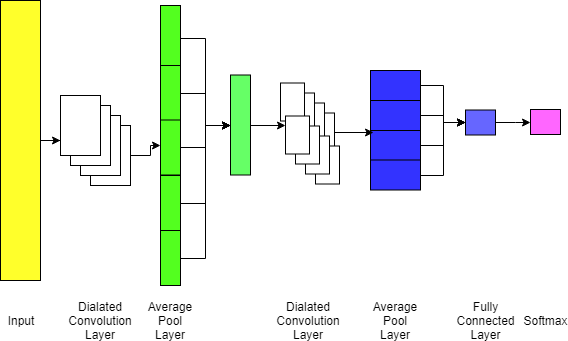
\includegraphics[width=10cm]{DCNN_architecture.png}
    \caption{Dilated Convoluted Neural Network architecture, implemented in this project.}
    \label{fig:DCNN}
\end{figure}

It consists of the input layer followed by a 1D Convolution Layer, with $16$ filters of size $64$. This layer is in fact a Dilated Convoluted Layer. This additional parameter to the convoluted layer represents spaces between each cell called a $dilation$. As an example, in one dimension a filter $w$ of size $3$ would compute over input $x$ the following: $w[0]*x[0] + w[1]*x[1] + w[2]*x[2]$. This is dilation of $0$. For dilation $1$ the filter would instead compute $w[0]*x[0] + w[1]*x[2] + w[2]*x[4]$; In other words there is a gap of 1 between the applications. This can be very useful in some settings to use in conjunction with 0-dilated filters because it allows you to merge spatial information across the inputs much more aggressively with fewer layers. For this model it was found that a dilation of $8$ worked best.

This convoluted layer is followed by a $50\%$ Dropout to help reduce over fitting, and an Average Pooling Layer of size $32$. This same architecture is then repeated with $64$ filters of size $16$ and $dilation$ factor of $2$, another $50\%$ Dropout, and an Average Pooling Layer of size $4$. The architecture for the model is completed with a fully connected layer with $softmax$ activation which outputs the probability among the 5 classes.

A categorical cross-entropy loss function defined by:
\[J(W, B) = -\sum_{i}\sum_{k} \mathbbm{1} (y^{(i)} = k) \log h_{w}(x^{(i)})\]
 
 where $W$ and $B$ are the matrices of weights and biases in our neural network respectively. $W$ and $B$ are optimized by the $adam$ optimizer.

% Model Accuracies
The accuracies of all model implementations are shown in Table 1. 
 \begin{table}[h!]
\centering
 \begin{tabular}{ |p{7.7cm}||p{3cm}|p{3cm} | }
 \hline
 \multicolumn{3}{|c|}{Accuracy} \\
 \hline
 Model                                                                      & Training Accuracy &Test Accuracy\\
 \hline
 SVM (Spotify audio features)                                  & 63.8\%                   &69.7\%          \\
  \hline
 Random Forest (Spotify audio features)                 & 92.8\%                   & 82\%            \\
 \hline
 FNN(Spotify audio features)                                    &96.2\%                   & 81\%            \\
 \hline
 CNN(MFCC)                                                            &97.5\%                   & 87\%            \\
 \hline
 SVM(features from CNN hidden layer 1)                 & 98\%                     & 85\%            \\
 \hline
 SVM(features from CNN hidden layer 2)                 & 99.7\%                  & 85\%            \\
 \hline
 Random Forest(features from CNN hidden layer 1)& 100\%                   & 86\%           \\
 \hline
 Random Forest(features from CNN hidden layer 2)& 100\%                   & 86\%           \\
 \hline
\end{tabular}
\caption{Accuracy of all classifier model implementations}
\label{table:1}
\end{table}

\section{Participants Contribution}
%Please list the name of the participants. For each participant explain in details the role he/she played in the project: explain which methods was implemented by which member, which dataset was processed by which member, which experimental results were generated by which members, etc.
Participants: Hyeonjung Ko, Yash Shetty\\

Hyeonjung Ko and Yash Shetty both worked on cleaning/modifying the dataset, implementing the models, and generating the experimental results. All models and results presented were first individually developed, then combined for best results. Such development include the models of SVM, Random Forest, FNN and CNN as well as their classification results.

\section{Refereces}
\begin{comment}

- http://cs229.stanford.edu/proj2018/report/19.pdf
- https://medium.com/@navdeepsingh_2336/identifying-the-genre-of-a-song-with-neural-networks-851db89c42f0
- https://towardsdatascience.com/using-cnns-and-rnns-for-music-genre-recognition-2435fb2ed6af
- https://towardsdatascience.com/machine-learning-and-music-classification-a-content-based-filtering-approach-f2c4eb13bade
- https://www.kaggle.com/zaheenhamidani/ultimate-spotify-tracks-db
- https://www.inference.vc/dilated-convolutions-and-kronecker-factorisation/
-http://cs231n.github.io/convolutional-networks/
\end{comment}
​
​
​
\vspace{10mm}
%** Please do not change the size of the fonts.
%** Please note that your submission must be at most 7 pages long, excluding references.
​
\end{document}
Collapse



